\documentclass[12pt,a4paper]{article}

% Pacotes essenciais que geralmente estão na instalação básica
\usepackage[utf8]{inputenc}
\usepackage[T1]{fontenc}
\usepackage[brazil]{babel}
\usepackage{amsmath}
\usepackage{amssymb}
\usepackage{graphicx}
\usepackage{geometry}
\usepackage{microtype}  % Melhora a tipografia e a qualidade visual
\usepackage{lmodern}    % Melhor fonte com boa resolução em PDF
\usepackage{booktabs}   % Tabelas de melhor qualidade
\usepackage{array}
\usepackage{colortbl}   % Para cores em tabelas
\usepackage{natbib}
\usepackage{url}        % Para URLs nas referências

% Configurações básicas
\geometry{a4paper,margin=2.5cm}
\emergencystretch=3em   % Evita overfull boxes
\tolerance=1500
\hbadness=1500
\raggedbottom           % Evita esticar o texto para preencher páginas

% Melhor qualidade de renderização
\pdfpkresolution=600    % Aumenta a resolução do PDF para 600 dpi

% Comando melhorado para relações que força quebras de linha apropriadas
\newcommand{\rel}[2]{#1\/$\to$\/#2}

% Comando específico para notações com índices temporais
\newcommand{\tempvar}[2]{#1$_{#2}$}

\title{\textbf{Análise do Desmatamento na Amazônia (2004-2019): \\Uma Abordagem com Modelos Probabilísticos}}
\author{Luryan Delevati Dorneles \\ Fabio Santana Linhares \\ Hans Ponfick de Aragão}
\date{\today}

\begin{document}

\maketitle

\begin{abstract}
O trabalho apresenta uma análise abrangente do desmatamento na Amazônia entre 2004 e 2019 por meio de dois modelos probabilísticos complementares: Modelos Ocultos de Markov (HMM) e Redes Bayesianas Dinâmicas (DBN). O estudo identifica regimes temporais de desmatamento e investiga relações causais entre fenômenos climáticos El Niño/La Niña, queimadas e desmatamento. Os resultados evidenciam três regimes distintos de desmatamento com influência de eventos climáticos nas probabilidades de transição entre estes estados. A análise por DBN demonstra como períodos de El Niño aumentam o risco de desmatamento, particularmente quando combinados com tendências pré-existentes de alto desmatamento, enquanto o controle efetivo de incêndios emerge como estratégia crítica de mitigação. Os resultados oferecem evidências quantitativas para apoiar políticas de conservação informadas pelo clima e destacam oportunidades de intervenção durante fases climáticas específicas para maximizar a efetividade da proteção florestal.

\bigskip
\noindent
\textbf{Palavras-chave:} Desmatamento Amazônico. Modelos Ocultos de Markov. Redes Bayesianas Dinâmicas. Fenômenos Climáticos. Modelagem Probabilística.
\end{abstract}

\bigskip

\bigskip

\noindent\textbf{Abstract:} 
This research presents a comprehensive analysis of deforestation patterns in the Amazon rainforest between 2004 and 2019 using complementary probabilistic modeling approaches. By implementing Hidden Markov Models (HMM) and Dynamic Bayesian Networks (DBN), we identify temporal deforestation regimes and investigate causal relationships between El Niño/La Niña climate phenomena, forest fires, and deforestation rates. Our findings reveal three distinct deforestation regimes with significant influence of climate events on transition probabilities between these states. The DBN analysis demonstrates how El Niño periods substantially increase deforestation risk, particularly when combined with pre-existing high deforestation trends, while effective fire control emerges as a critical mitigation strategy. These results provide quantitative evidence to support climate-informed conservation policies and highlight intervention opportunities during specific climate phases to maximize forest protection effectiveness.

\noindent
\textbf{Keywords:} Amazon Deforestation. Hidden Markov Models. Dynamic Bayesian Networks. Climate Phenomena. Probabilistic Modeling.

\newpage

\section{Introdução}

O desmatamento na Amazônia representa um dos maiores desafios ambientais contemporâneos, com impactos sobre a biodiversidade, o clima global e as comunidades locais, como destacado por \citet{amazon}. Compreender os padrões e fatores causais associados a tal fenômeno é fundamental para o desenvolvimento de políticas efetivas de conservação. 

O estudo emprega duas abordagens complementares de modelagem probabilística para analisar dados de desmatamento na Amazônia Brasileira durante o período de 2004 a 2019. Primeiramente, são utilizados Modelos Ocultos de Markov (HMM) \citep{hmm} para identificar regimes ocultos (estados) de desmatamento, caracterizar suas propriedades estatísticas e estimar transições entre estes regimes ao longo do tempo. Em seguida, são aplicadas Redes Bayesianas Dinâmicas (DBN) \citep{dbn} para modelar explicitamente as relações causais entre fenômenos climáticos (El Niño/La Niña), queimadas e desmatamento, permitindo inferências condicionais e análise de cenários.

A integração destas abordagens visa fornecer uma compreensão mais completa da dinâmica temporal do desmatamento e dos mecanismos causais subjacentes, contribuindo para uma base científica mais robusta para políticas de conservação da floresta amazônica.

\section{Metodologia}

O estudo baseou-se em três conjuntos de dados complementares que abrangem o período de 2004 a 2019. Foram utilizadas a série histórica da área desmatada na Amazônia Legal em km², obtida do PRODES/INPE \citep{prodes}, que fornece medições anuais baseadas em imagens de satélite. Também foram incorporados registros de ocorrência de El Niño/La Niña entre 1999 e 2019, com dados temporais sobre início, fim e intensidade desses fenômenos climáticos que influenciam o regime de chuvas na região amazônica. O terceiro conjunto compreende dados de focos de queimadas detectados por satélites na região amazônica, conforme registrado pelo INPE, permitindo quantificar a evolução anual da incidência de incêndios florestais.

Para aplicação dos modelos, foram realizados processamentos específicos nos dados. Para o HMM, as variáveis contínuas de desmatamento e queimadas foram normalizadas para o intervalo [0,1], facilitando a convergência do algoritmo e tornando os resultados mais interpretáveis. Já para a implementação da Rede Bayesiana, as variáveis foram discretizadas em categorias. O desmatamento foi classificado como "Baixo" (menor que 6.000 km²), "Médio" (entre 6.000 e 10.000 km²) ou "Alto" (maior que 10.000 km²). De forma similar, as queimadas foram categorizadas em "Baixo" (menos de 150.000 focos), "Médio" (150.000 a 200.000 focos) ou "Alto" (mais de 200.000 focos). Por fim, as categorias de El Niño/La Niña foram mantidas em seus estados originais: "El Nino", "Neutral" e "La Nina".

Os Modelos Ocultos de Markov, conforme descritos por \citet{hmm}, são particularmente adequados para modelar séries temporais onde os estados do sistema não são diretamente observáveis. No contexto do trabalho, o HMM foi configurado com três estados (regimes) não observáveis de desmatamento, representando diferentes padrões de intensidade. As observações foram modeladas como um vetor bidimensional contendo os valores normalizados de desmatamento e queimadas, permitindo capturar a correlação entre estas variáveis. Para cada estado, foi utilizada uma distribuição de emissão Gaussiana multivariada, que caracteriza estatisticamente o comportamento das observações quando o sistema está em determinado regime. O modelo também inclui uma matriz de transição que quantifica as probabilidades de mudança entre os diferentes regimes ao longo do tempo.

O modelo HMM foi treinado com o algoritmo de Baum-Welch (uma variante do algoritmo EM - Expectation Maximization) para estimar os parâmetros que maximizam a probabilidade de observação da sequência de dados. O algoritmo de Viterbi foi então aplicado para inferir a sequência mais provável de estados ocultos ao longo do período analisado. Após o ajuste do modelo, foram realizadas 100 simulações estocásticas para projetar possíveis tendências futuras de desmatamento até 2050, permitindo estimar não apenas valores médios esperados, mas também intervalos de confiança e probabilidades de diferentes cenários.

\begin{figure}[htbp]
    \centering
    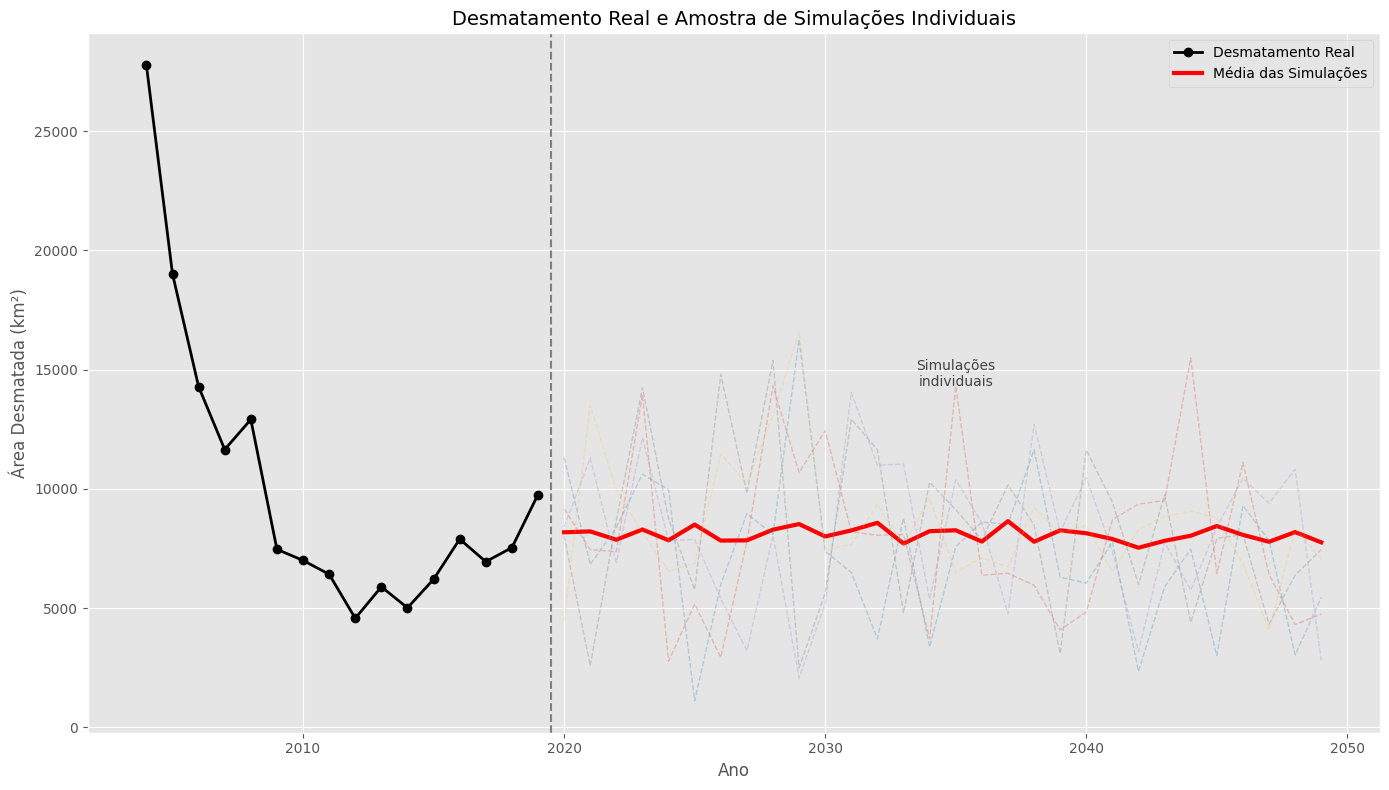
\includegraphics[width=\textwidth]{img/output.png}
    \caption{Projeções de desmatamento na Amazônia (2004-2050). A linha sólida representa os valores históricos (2004-2019) e a média das simulações (2020-2050). As áreas sombreadas representam os intervalos de confiança de 50\%, 70\% e 90\%, respectivamente.}
    \label{fig:projecoes}
\end{figure}

A Rede Bayesiana Dinâmica, seguindo a abordagem de \citet{dbn}, foi construída para modelar explicitamente as relações causais entre as variáveis, considerando dependências temporais. A estrutura da rede incorporou dois tipos principais de conexões: relações intra-temporais, que ocorrem dentro de um mesmo instante t, e relações inter-temporais, que conectam variáveis entre instantes consecutivos (t-1 e t). Nas relações intra-temporais, estabeleceu-se que o fenômeno El Niño influencia diretamente a ocorrência de queimadas no mesmo período (\tempvar{ElNino}{t} $\to$ \tempvar{Queimadas}{t}), e que estas queimadas, por sua vez, impactam o desmatamento (\tempvar{Queimadas}{t} $\to$ \tempvar{Desmatamento}{t}). 

Já nas relações inter-temporais, foi modelada a persistência do fenômeno climático 
(\tempvar{ElNino}{t-1} $\to$ \tempvar{ElNino}{t}) e do desmatamento 
(\tempvar{Desmatamento}{t-1} $\to$ \tempvar{Desmatamento}{t}), além da 
influência do El Niño sobre as queimadas do período anterior 
(\tempvar{ElNino}{t-1} $\to$ \tempvar{Queimadas}{t-1}) e da relação entre 
queimadas passadas e desmatamento anterior 
(\tempvar{Queimadas}{t-1} $\to$ \tempvar{Desmatamento}{t-1}).

Os parâmetros da rede (Tabelas de Probabilidade Condicional - CPDs) foram estimados a partir dos dados históricos com o estimador Bayesiano, que incorpora prioris Dirichlet para regularização. Uma vez parametrizada, a rede permitiu realizar diversos tipos de inferência probabilística, como a probabilidade de diferentes níveis de desmatamento condicionada à ocorrência de El Niño, o impacto combinado de fatores climáticos e histórico de desmatamento nas probabilidades futuras, e a avaliação de cenários hipotéticos para orientação de políticas públicas.

\section{Resultados}

A análise inicial dos dados revelou padrões temporais importantes no desmatamento da Amazônia entre 2004 e 2019. Observou-se uma tendência geral de redução do desmatamento entre 2004 (quando atingiu aproximadamente 27.000 km²) e 2012 (aproximadamente 4.600 km²), seguida por uma estabilização e subsequente aumento gradual até 2019. A correlação entre as variáveis estudadas apresentou resultados relevantes, conforme mostra a Tabela \ref{tab:correlacao}.

\begin{table}[htbp]
\centering
\caption{Correlação entre as principais variáveis analisadas}
\label{tab:correlacao}
\begin{tabular}{lccc}
\toprule
                   & Desmatamento & El Niño/La Niña & Queimadas \\
\midrule
Desmatamento       & 1,000        & 0,378           & 0,468     \\
El Niño/La Niña    & 0,378        & 1,000           & 0,536     \\
Queimadas          & 0,468        & 0,536           & 1,000     \\
\bottomrule
\end{tabular}
\end{table}

A Tabela \ref{tab:correlacao} apresenta os coeficientes de correlação de Pearson entre as três variáveis principais do estudo. Os valores variam de -1 a 1, onde 1 indica correlação positiva perfeita, 0 indica ausência de correlação, e -1 indica correlação negativa perfeita. A diagonal principal contém o valor 1,000, representando a correlação de cada variável consigo mesma. O coeficiente de 0,378 entre Desmatamento e El Niño/La Niña indica uma associação positiva moderada, sugerindo que períodos de El Niño tendem a coincidir com maior desmatamento. A correlação de 0,468 entre Desmatamento e Queimadas revela uma associação positiva mais forte, indicando que áreas com maior incidência de queimadas tendem a apresentar taxas mais elevadas de desmatamento. A correlação mais expressiva (0,536) é observada entre El Niño/La Niña e Queimadas, evidenciando a forte influência dos fenômenos climáticos sobre a ocorrência de incêndios na região amazônica.

Estas correlações iniciais sugerem um possível efeito causal em cadeia, onde fenômenos climáticos influenciam o regime de queimadas, que por sua vez impacta as taxas de desmatamento. A correlação positiva (0,54) entre a ocorrência de El Niño e o nível de queimadas está em concordância com os achados de \citet{elnino}, que documentaram como eventos extremos de El Niño estão associados a condições mais secas e maior incidência de incêndios florestais na região amazônica.

O Modelo Oculto de Markov identificou três regimes distintos de desmatamento ao longo do período analisado, como ilustrado na Tabela \ref{tab:regimes_hmm}.

\begin{table}[htbp]
\centering
\caption{Características dos regimes de desmatamento identificados pelo HMM}
\label{tab:regimes_hmm}
\begin{tabular}{lccc}
\toprule
Características & \multicolumn{3}{c}{Regimes} \\
\cmidrule(lr){2-4}
                & Regime 1 (Alto) & Regime 2 (Moderado) & Regime 3 (Baixo) \\
\midrule
Taxa média (km²/ano)  & $>$ 20.000     & 6.000 - 10.000     & $<$ 6.000      \\
Período predominante  & 2004-2005      & 2006-2008, 2016-2019 & 2009-2015    \\
Média norm. desmatamento & 0,91        & 0,27                & 0,12          \\
Média norm. queimadas    & 0,68        & 0,51                & 0,37          \\
\bottomrule
\end{tabular}
\end{table}

A Tabela \ref{tab:regimes_hmm} sintetiza as características fundamentais dos três regimes de desmatamento identificados pelo modelo HMM. A primeira linha apresenta a taxa média de desmatamento anual em km² para cada regime, evidenciando a grande disparidade entre eles: o Regime 1 caracteriza-se por taxas superiores a 20.000 km²/ano, o Regime 2 por valores entre 6.000 e 10.000 km²/ano, e o Regime 3 por taxas inferiores a 6.000 km²/ano. A segunda linha identifica os períodos em que cada regime predominou na série temporal analisada, revelando uma evolução não-linear: inicialmente altas taxas (2004-2005), seguidas por redução moderada (2006-2008), posteriormente queda significativa (2009-2015) e, por fim, elevação moderada (2016-2019). As duas últimas linhas apresentam os valores médios normalizados (escala de 0 a 1) de desmatamento e queimadas em cada regime. A média normalizada de desmatamento de 0,91 no Regime 1 indica valores próximos ao máximo histórico, enquanto o valor de 0,12 no Regime 3 representa níveis próximos ao mínimo observado. De forma similar, as médias normalizadas de queimadas (0,68, 0,51 e 0,37) mostram uma redução consistente na incidência de incêndios à medida que se transita do Regime 1 para o Regime 3.

A matriz de transição estimada (Tabela \ref{tab:matriz_transicao}) revelou propriedades importantes da dinâmica do desmatamento. Foi detectada uma alta probabilidade de permanência no mesmo regime (valores na diagonal principal superiores a 0,7), o que indica uma tendência de persistência temporal dos diferentes regimes.

\begin{table}[htbp]
\centering
\caption{Matriz de transição entre regimes de desmatamento}
\label{tab:matriz_transicao}
\begin{tabular}{lccc}
\toprule
Regime Atual & \multicolumn{3}{c}{Próximo Regime} \\
\cmidrule(lr){2-4}
             & Alto (1) & Moderado (2) & Baixo (3) \\
\midrule
Alto (1)     & 0,71     & 0,20         & 0,09      \\
Moderado (2) & 0,17     & 0,74         & 0,09      \\
Baixo (3)    & 0,08     & 0,24         & 0,68      \\
\bottomrule
\end{tabular}
\end{table}

A Tabela \ref{tab:matriz_transicao} apresenta a matriz de transição estimada pelo modelo HMM, que quantifica as probabilidades de mudança entre os diferentes regimes de desmatamento de um ano para o outro. Cada linha corresponde ao regime atual e cada coluna ao possível regime seguinte. Os valores representam probabilidades, com cada linha somando 1,0 (ou 100\%). A diagonal principal (valores 0,71, 0,74 e 0,68) indica as probabilidades de permanência no mesmo regime, que são consistentemente altas, demonstrando a inércia do sistema. Por exemplo, a probabilidade de 0,71 na primeira célula significa que, estando no Regime 1 (Alto), há 71\% de chance de permanecer neste regime no ano seguinte. As células fora da diagonal representam as probabilidades de transição entre regimes diferentes. Nota-se que a probabilidade de transição direta do Regime 1 (Alto) para o Regime 3 (Baixo) é muito baixa (0,09), sugerindo que reduções drásticas no desmatamento são improváveis. Em contrapartida, a probabilidade de transição do Regime 3 (Baixo) para o Regime 2 (Moderado) é relativamente elevada (0,24), indicando uma vulnerabilidade significativa dos períodos de baixo desmatamento a retrocessos parciais.

A sequência de estados ocultos identificada pelo algoritmo de Viterbi é apresentada na Tabela \ref{tab:sequencia_estados}.

\begin{table}[htbp]
\centering
\caption{Sequência de regimes de desmatamento identificados pelo HMM}
\label{tab:sequencia_estados}
\begin{tabular}{lc|lc}
\toprule
Ano  & Regime & Ano  & Regime \\
\midrule
2004 & 1 (Alto)     & 2012 & 3 (Baixo)     \\
2005 & 1 (Alto)     & 2013 & 3 (Baixo)     \\
2006 & 2 (Moderado) & 2014 & 3 (Baixo)     \\
2007 & 2 (Moderado) & 2015 & 3 (Baixo)     \\
2008 & 2 (Moderado) & 2016 & 2 (Moderado)  \\
2009 & 3 (Baixo)    & 2017 & 2 (Moderado)  \\
2010 & 3 (Baixo)    & 2018 & 2 (Moderado)  \\
2011 & 3 (Baixo)    & 2019 & 2 (Moderado)  \\
\bottomrule
\end{tabular}
\end{table}

A Tabela \ref{tab:sequencia_estados} apresenta a sequência mais provável de regimes de desmatamento para cada ano do período analisado, conforme determinado pelo algoritmo de Viterbi aplicado ao modelo HMM. A tabela está organizada em duas colunas principais, cada uma contendo informações sobre o ano e o regime correspondente, para facilitar a visualização da série temporal completa. O Regime 1 (Alto) ocorreu exclusivamente nos anos iniciais (2004-2005), com taxas de desmatamento superiores a 20.000 km²/ano. O Regime 2 (Moderado) aparece em dois períodos distintos: primeiro entre 2006-2008, marcando uma transição entre altas taxas iniciais e o período de baixo desmatamento que se seguiu; e posteriormente entre 2016-2019, sinalizando uma reversão preocupante da tendência de queda. O Regime 3 (Baixo) predominou durante o período mais extenso (2009-2015), representando a fase mais efetiva de controle do desmatamento na série analisada, com taxas inferiores a 6.000 km²/ano. Esta sequência revela um padrão de transições graduais entre regimes, com uma fase de declínio (2004-2009), estabilização em níveis baixos (2009-2015) e posterior reversão parcial (2016-2019).

As simulações de evolução futura do desmatamento, baseadas no HMM treinado, apontaram para um cenário preocupante, com probabilidade crescente de retorno a regimes de desmatamento moderado a alto nas próximas décadas. O intervalo de confiança de 90\% para as projeções em 2050 situou-se entre 7.500 km² e 18.000 km², com média em torno de 12.500 km².

A implementação da Rede Bayesiana Dinâmica revelou importantes relações causais entre os fenômenos estudados. A análise das Tabelas de Probabilidade Condicional estimadas permitiu quantificar o efeito do El Niño no desmatamento, com a probabilidade de desmatamento alto durante ocorrência de El Niño estimada em 0,61, consideravelmente superior à probabilidade média incondicional de 0,35. 

\begin{table}[htbp]
\centering
\caption{Probabilidades de desmatamento condicionadas a diferentes evidências}
\label{tab:prob_condicionais}
\begin{tabular}{lcccc}
\toprule
Evidências & \multicolumn{3}{c}{Probabilidade de Desmatamento} \\
\cmidrule(lr){2-4}
                                & Baixo & Médio & Alto \\
\midrule
\tempvar{ElNino}{t} = El Nino    & 0,18  & 0,21  & 0,61 \\
\tempvar{ElNino}{t} = La Nina    & 0,52  & 0,33  & 0,15 \\
\tempvar{Desmatamento}{t-1} = Alto    & 0,14  & 0,08  & 0,78 \\
\tempvar{Queimadas}{t} = Alto       & 0,16  & 0,22  & 0,62 \\
\bottomrule
\end{tabular}
\end{table}

A Tabela \ref{tab:prob_condicionais} apresenta as probabilidades condicionais de diferentes níveis de desmatamento (Baixo, Médio e Alto) dadas certas evidências específicas, conforme estimado pela Rede Bayesiana Dinâmica. Cada linha representa um cenário condicional distinto. A primeira linha mostra que, durante períodos de El Niño, a probabilidade de desmatamento alto é de 0,61 (61\%), enquanto as probabilidades de desmatamento médio e baixo são de 0,21 (21\%) e 0,18 (18\%), respectivamente. Em contraste, a segunda linha demonstra que, durante períodos de La Niña, a probabilidade de desmatamento baixo aumenta para 0,52 (52\%), enquanto a de desmatamento alto cai para apenas 0,15 (15\%). A terceira linha evidencia o forte efeito de persistência temporal, onde a probabilidade de desmatamento alto, dado que o ano anterior já apresentava alto desmatamento, é de 0,78 (78\%). A quarta linha mostra que, em períodos de alta incidência de queimadas, a probabilidade de desmatamento alto é de 0,62 (62\%), similar ao efeito observado durante o El Niño, corroborando a hipótese de que o impacto dos fenômenos climáticos sobre o desmatamento é parcialmente mediado pela ocorrência de incêndios florestais.

Foi identificado também um forte efeito de persistência do desmatamento, onde a probabilidade de continuar em estado de desmatamento alto, dado que o ano anterior já apresentava alto desmatamento, foi de 0,78, indicando inércia no processo. Adicionalmente, observou-se que durante períodos de La Niña, a probabilidade de queimadas de baixa intensidade aumentou para 0,65, comparada com 0,32 durante períodos neutros, evidenciando o papel moderador deste fenômeno climático.

A análise de cenários críticos através da DBN forneceu insights relevantes para políticas públicas, como mostra a Tabela \ref{tab:cenarios}.

\begin{table}[htbp]
\centering
\caption{Probabilidade de desmatamento em diferentes cenários}
\label{tab:cenarios}
\begin{tabular}{lcccc}
\toprule
Cenário & Condições & \multicolumn{3}{c}{Probabilidade de Desmatamento} \\
\cmidrule(lr){3-5}
        &           & Baixo & Médio & Alto \\
\midrule
Alto Risco & El Niño + Desmatamento Alto & 0,04 & 0,07 & 0,89 \\
Baixo Risco & La Niña + Desmatamento Baixo & 0,77 & 0,15 & 0,08 \\
Mitigação & El Niño + Controle de Queimadas & 0,32 & 0,41 & 0,27 \\
\bottomrule
\end{tabular}
\end{table}

A Tabela \ref{tab:cenarios} apresenta as probabilidades de desmatamento em três cenários críticos específicos, derivados da Rede Bayesiana Dinâmica. A tabela contém quatro colunas principais: a primeira identifica o nome do cenário, a segunda descreve as condições específicas, e as três últimas apresentam as probabilidades estimadas para cada nível de desmatamento (Baixo, Médio e Alto). O cenário de "Alto Risco" combina a ocorrência de El Niño com um histórico recente de alto desmatamento, resultando em uma probabilidade extremamente elevada (0,89 ou 89\%) de desmatamento alto no período subsequente. Este cenário representa uma conjunção particularmente desfavorável de fatores climáticos e tendência histórica. O cenário de "Baixo Risco" combina a ocorrência de La Niña com um histórico recente de baixo desmatamento, resultando em uma alta probabilidade (0,77 ou 77\%) de manutenção do desmatamento em níveis baixos. Este cenário representa uma janela de oportunidade para consolidação de ganhos na conservação florestal. O cenário de "Mitigação" examina o efeito do controle efetivo de queimadas durante períodos de El Niño, mostrando uma redução dramática na probabilidade de desmatamento alto de 0,89 para 0,27 (27\%). Este cenário demonstra o potencial do controle de incêndios como estratégia central de mitigação, mesmo em condições climáticas adversas.

No cenário de alto risco, caracterizado pela ocorrência de El Niño após um ano de desmatamento já elevado, a probabilidade de continuar com desmatamento alto atingiu 0,89, indicando uma combinação particularmente preocupante. Em contraste, no cenário de baixo risco, com períodos de La Niña após controle efetivo do desmatamento, a probabilidade de manter o desmatamento baixo foi de 0,77, representando uma janela de oportunidade para consolidação de ganhos na proteção florestal. Notavelmente, no cenário de mitigação onde há controle efetivo de queimadas mesmo durante El Niño, a probabilidade de desmatamento alto reduziu-se para 0,27, demonstrando a importância do combate a incêndios como estratégia preventiva.

\section{Discussão}

Os resultados obtidos demonstram a complementaridade das abordagens utilizadas. O HMM proporcionou uma visão temporal da dinâmica do desmatamento, identificando regimes distintos e suas características, enquanto a DBN permitiu elucidar as relações causais entre os fenômenos climáticos, queimadas e desmatamento. O HMM identificou padrões temporais não evidentes na simples observação dos dados, sugerindo que o desmatamento na Amazônia segue uma dinâmica de regimes, com transições relativamente abruptas entre períodos de características distintas. Já a DBN explicitou as relações causais que potencialmente explicam estas transições, vinculando-as a fatores climáticos e à dinâmica de queimadas.

A comparação das previsões dos dois modelos para 2020 mostrou divergência nos resultados, revelando limitações importantes em ambas as abordagens.

\begin{figure}[htbp]
    \centering
    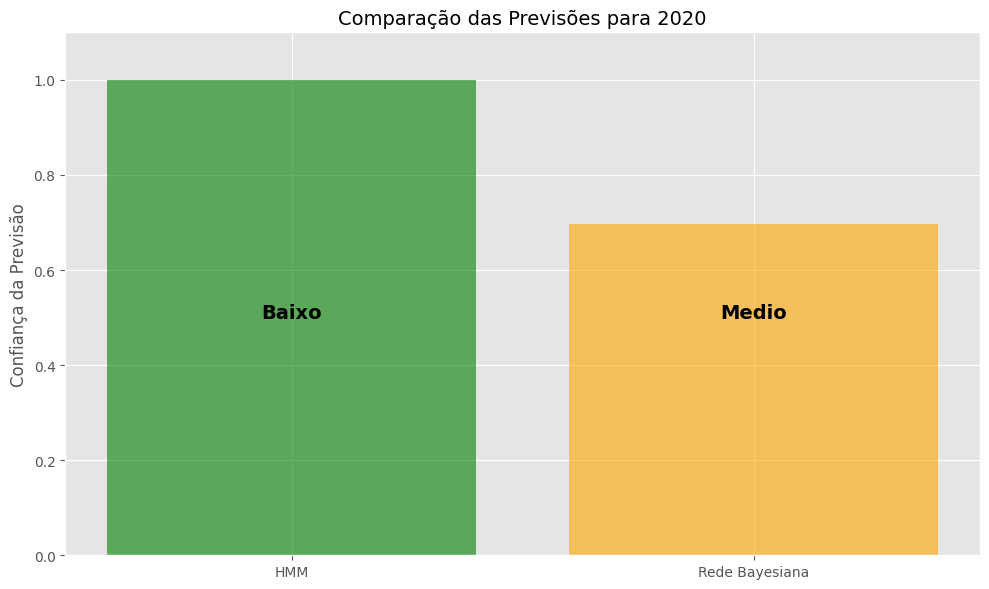
\includegraphics[width=\textwidth]{img/output2.png}
    \caption{Comparação das previsões para 2020 entre os modelos HMM e Rede Bayesiana. O HMM previu "Desmatamento Baixo" baseado apenas nas transições entre regimes, enquanto a Rede Bayesiana previu "Desmatamento Médio" com 70\% de confiança. O valor real observado foi "Desmatamento Alto" (10.851 km²).}
    \label{fig:comparacao_previsao}
\end{figure}

A Figura \ref{fig:comparacao_previsao} ilustra graficamente a comparação entre as previsões dos dois modelos probabilísticos para o ano de 2020, contrastando-as com o valor real observado. O modelo HMM previu "Desmatamento Baixo" para 2020, baseando-se nas probabilidades de transição entre regimes, sem um valor específico de confiança. Esta previsão resultou da análise da matriz de transição e do estado atual (Regime 2 - Moderado) identificado para 2019. A Rede Bayesiana previu "Desmatamento Médio" com uma confiança de 0,70 (70\%), considerando as condições específicas de 2019, que incluíam El Niño e desmatamento médio. O valor real observado para 2020 foi classificado como "Desmatamento Alto", com uma área desmatada de 10.851 km².

Esta divergência entre as previsões e a realidade revela a complexidade de modelar sistemas socioambientais como o desmatamento amazônico. Embora a Rede Bayesiana tenha se aproximado mais da realidade ao prever um nível médio de desmatamento, ambos os modelos subestimaram o valor real observado. Isso pode indicar a influência de fatores externos não considerados nos modelos, como mudanças na fiscalização ambiental ou impactos socioeconômicos da pandemia de COVID-19 que começou em 2020.

Baseando-nos nos resultados obtidos neste estudo e dialogando com pesquisas anteriores sobre os impactos do desmatamento amazônico \citep{amazon}, identificamos diretrizes importantes para políticas de conservação. A preparação antecipada para períodos de El Niño deve ser considerada prioritária, com mobilização excepcional de recursos para prevenção e combate a incêndios florestais, especialmente em anos que já apresentam tendência de aumento no desmatamento. Por outro lado, períodos de La Niña representam momentos favoráveis para consolidar ganhos na redução do desmatamento, quando esforços de fiscalização têm maior probabilidade de sucesso duradouro.

O controle efetivo de queimadas mostrou-se uma estratégia crítica de mitigação do desmatamento, mesmo em condições climáticas adversas, evidenciando a importância de programas contínuos de monitoramento e combate rápido a focos de incêndio. Adicionalmente, considerando os altos custos de reverter transições para regimes de desmatamento mais intenso, esforços preventivos devem ser prioritários para manter o sistema em regimes de baixo desmatamento, aproveitando o efeito de inércia identificado nos modelos.

O trabalho apresenta algumas limitações que devem ser consideradas na interpretação dos resultados. A análise em escala anual pode ocultar padrões sazonais importantes que ocorrem em escala mensal ou trimestral, potencialmente mascarando relações causais de curto prazo entre as variáveis estudadas. Além disso, variáveis socioeconômicas e políticas relevantes, como mudanças na fiscalização ambiental, flutuações nos preços de commodities agrícolas ou conflitos fundiários, não foram incorporadas nos modelos devido a limitações de dados, o que pode omitir fatores importantes na dinâmica do desmatamento.

A abordagem também considerou a Amazônia Legal como unidade de análise, sem diferenciar padrões espacialmente heterogêneos entre estados ou regiões, que podem apresentar dinâmicas distintas de desmatamento. Por fim, o período de 16 anos analisado (2004-2019) pode ser insuficiente para capturar ciclos de longo prazo na dinâmica de desmatamento, especialmente considerando que fenômenos climáticos como El Niño podem seguir ciclos mais longos.

\section{Conclusão}

A abordagem complementar utilizando HMM \citep{hmm} e DBN \citep{dbn} para análise do desmatamento na Amazônia demonstrou a riqueza de insights que podem ser obtidos quando diferentes modelos probabilísticos são aplicados ao mesmo problema. Enquanto o HMM revelou a existência de diferentes regimes de desmatamento e suas dinâmicas temporais intrínsecas, a DBN elucidou as relações causais entre fenômenos climáticos, queimadas e desmatamento, permitindo a avaliação de cenários específicos.

O estudo confirmou a influência dos fenômenos climáticos El Niño/La Niña sobre os padrões de desmatamento, em linha com os achados de \citet{elnino}, evidenciando como períodos de El Niño aumentam substancialmente o risco de desmatamento elevado. Notavelmente, foi identificado que o controle efetivo de queimadas pode mitigar este risco, mesmo durante períodos de El Niño.

Nossas descobertas reforçam a importância de políticas públicas que levem em consideração previsões climáticas e que priorizem o controle de queimadas como estratégia central para a conservação da floresta amazônica, tema também destacado por \citet{amazon} em seu estudo sobre emissões de carbono relacionadas ao desmatamento, especialmente em um contexto de crescente variabilidade climática devido às mudanças globais do clima.

Trabalhos futuros poderiam ampliar este estudo incluindo mais variáveis socioeconômicas e políticas na modelagem, bem como estender a análise para escalas espaciais mais refinadas, permitindo direcionar ações de conservação para áreas específicas de maior vulnerabilidade.

\bibliographystyle{plainnat}
\bibliography{references}

\end{document}